\chapter{}

\noindent For ChatGPT Webpage that allows connecting to a robot:

\noindent\href{https://github.com/Terramet/ChatNao}{https://github.com/Terramet/ChatNao}

\noindent The same thing as above with ChatGPT having the ability to access realtime apis and runs in Python instead:

\noindent \href{https://github.com/Terramet/ChatNaoPython}{https://github.com/Terramet/ChatNaoPython}

\noindent For the standalone Watson Sentiment analysis:

\noindent \href{https://github.com/Terramet/WatsonSentimentAnalysis}{https://github.com/Terramet/WatsonSentimentAnalysis}

\noindent Standalone facial emotion detection:

\noindent \href{https://github.com/Terramet/MPhilFacialEmotionDetection}{https://github.com/Terramet/MPhilFacialEmotionDetection}

\noindent For the ChatGPT results, including reponse times and the actual response:

\noindent \href{https://github.com/Terramet/MPhilDataStorage/tree/main/ChatGPTTests}{https://github.com/Terramet/MPhilDataStorage/tree/main/ChatGPTTests}

\noindent For all the models used for testing the facial emotion recognition, yolo, vgg16, resnet50 and mobilenetv2:

\noindent \href{https://github.com/Terramet/MPhilDataStorage/tree/main/Models}{https://github.com/Terramet/MPhilDataStorage/tree/main/Models}

\noindent For all the results from every detected face in the Exp\_W dataset:

\noindent \href{https://github.com/Terramet/MPhilDataStorage/tree/main/results_closest_face_pc}{https://github.com/Terramet/MPhilDataStorage/tree/main/results\_closest\_face\_pc}

\noindent For all the results from every detected face in the Exp\_W dataset on the robot:

\noindent \href{https://github.com/Terramet/MPhilDataStorage/tree/main/results_closest_face_robot}{https://github.com/Terramet/MPhilDataStorage/tree/main/results\_closest\_face\_robot}
%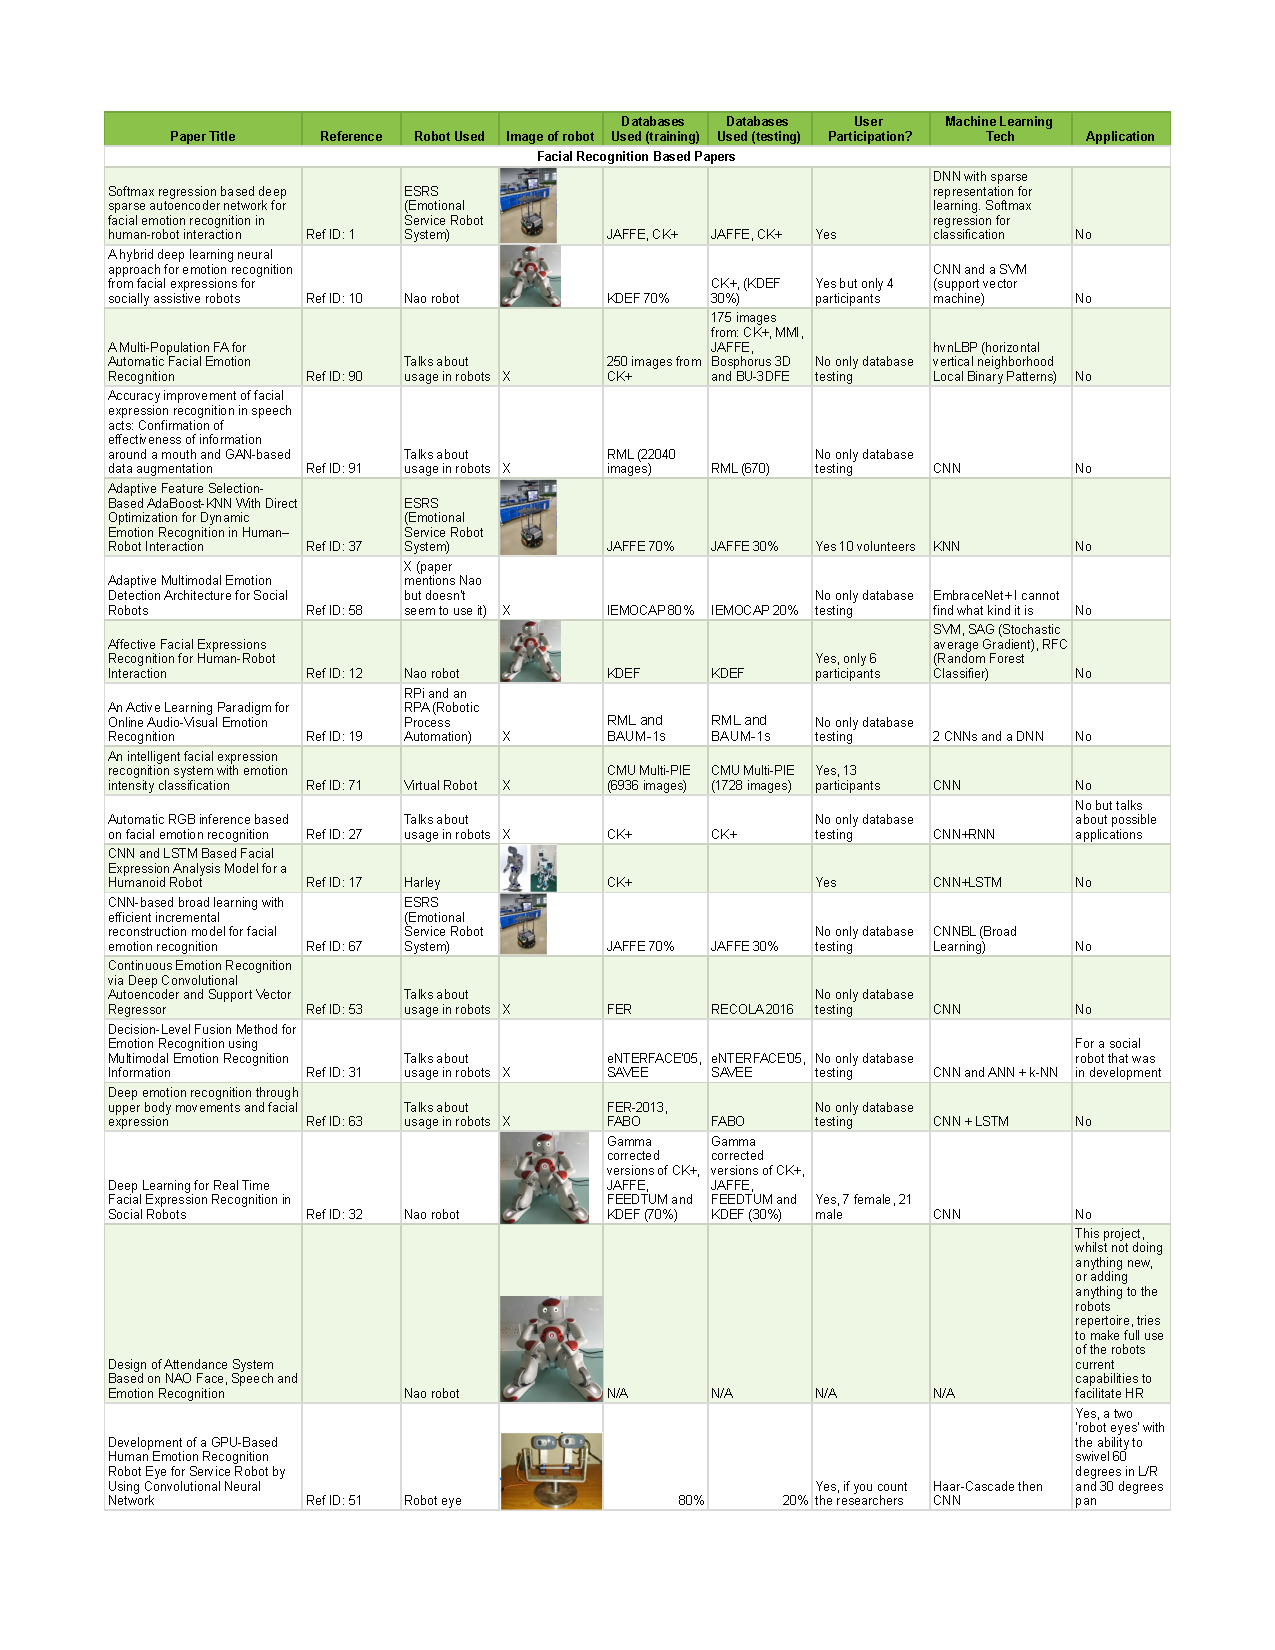
\includepdf[pages=-]{Appendix1/paperTable.pdf}

\noindent For a video showing the different voices available through IBM Watson

\noindent \href{https://youtube.com/shorts/Qqz03HE4MFg}{https://youtube.com/shorts/Qqz03HE4MFg}